\documentclass[12pt,a4paper]{article}
\usepackage{hyperref} % Use the Charter font for the document text
%\usepackage[UTF8]{ctex}
\usepackage{fullpage}
\usepackage{amsfonts,amssymb,amsmath}


\newcommand{\bA}{\ensuremath{\mathbb{A}}}
\newcommand{\bB}{\ensuremath{\mathbb{B}}}
\newcommand{\bC}{\ensuremath{\mathbb{C}}}
\newcommand{\bD}{\ensuremath{\mathbb{D}}}
\newcommand{\bE}{\ensuremath{\mathbb{E}}}
\newcommand{\bF}{\ensuremath{\mathbb{F}}}
\newcommand{\bG}{\ensuremath{\mathbb{G}}}
\newcommand{\bH}{\ensuremath{\mathbb{H}}}
\newcommand{\bI}{\ensuremath{\mathbb{I}}}
\newcommand{\bJ}{\ensuremath{\mathbb{J}}}
\newcommand{\bK}{\ensuremath{\mathbb{K}}}
\newcommand{\bL}{\ensuremath{\mathbb{L}}}
\newcommand{\bM}{\ensuremath{\mathbb{M}}}
\newcommand{\bN}{\ensuremath{\mathbb{N}}}
\newcommand{\bO}{\ensuremath{\mathbb{O}}}
\newcommand{\bP}{\ensuremath{\mathbb{P}}}
\newcommand{\bQ}{\ensuremath{\mathbb{Q}}}
\newcommand{\bR}{\ensuremath{\mathbb{R}}}
\newcommand{\bS}{\ensuremath{\mathbb{S}}}
\newcommand{\bT}{\ensuremath{\mathbb{T}}}
\newcommand{\bU}{\ensuremath{\mathbb{U}}}
\newcommand{\bV}{\ensuremath{\mathbb{V}}}
\newcommand{\bW}{\ensuremath{\mathbb{W}}}
\newcommand{\bX}{\ensuremath{\mathbb{X}}}
\newcommand{\bY}{\ensuremath{\mathbb{Y}}}
\newcommand{\bZ}{\ensuremath{\mathbb{Z}}}



\newtheorem{lemma}{Lemma}[section]
\newtheorem{conjecture}[lemma]{Conjecture} 
\newtheorem{corollary}[lemma]{Corollary} 
\newtheorem{theorem}[lemma]{Theorem} 
\newtheorem{definition}[lemma]{Definition} 
\newtheorem{question}[lemma]{Question} 
\newtheorem{proposition}[lemma]{Proposition} 

\usepackage{graphicx}


\begin{document}\thispagestyle{empty}

\centerline{\Large \bf Homework 4: Due at class on March 31}

 
\vspace{.5cm}
\noindent 1. Let  $\omega$ be the $n$-form on the space $\bR^{n+1}\backslash\{0\}$ defined by 
$$
\omega=\frac{1}{|x|^{n+1}}\sum_{i=1}^{n+1}(-1)^{i-1}x_idx_1\wedge \cdots \wedge \widehat{dx_i} \wedge \cdots \wedge dx_{n+1}~,
$$
where $|x|=(x_1^2+\cdots x_{n+1}^2)^{1/2}$.
Let $\iota:S^n\hookrightarrow \bR^{n+1}$ be the unit sphere in $\bR^{n+1}$. Show that $\iota^* \omega$ is the generator of $n$-the de Rham cohomology $H^n_{dR}(S^n)$ of the $n$-sphere. In fact, the de Rham cohomology of $S^n$ is 
$$
H^k_{dR}(S^n)=\left\{\begin{array}{l} \bR \quad k=0,~n \\ 0 ~ \quad  \textrm{otherwise}\end{array}\right.~.
$$
 
\vspace{.5cm}
\noindent 2. Let $\iota:S^2 \hookrightarrow \bR^3$ be the inclusion of the 2-sphere with unit radius.  Let $g:ds^2=\sum_{i=1}^3dx^i\otimes dx^i$ be the standard metric of $\bR^3$. Find the induced metric $\iota^* g$ on $S^2$ in terms of the polar coordinate of $\bR^3$.
\begin{align}
x_1&=r\sin\theta \cos\phi\cr
x_2&=r\sin\theta \sin\phi\cr
x_3&=r\cos\theta\nonumber
\end{align}
 
\vspace{.5cm}
\noindent 3. Let $ds^2=-dt^2+dx^2+dy^2$ be the Minkowski metric on $\bR^3$ and $-t^2+x^2+y^2=-1$ for $t>0$ be the space-like surface (hyperboloid $\mathbf{S}$). (See Figure 1.) Find the induced metric on the hyperboloid $S$ in terms of the polar coordinate
\begin{align}
t&=r \cosh \rho  \cr
x&=r\sinh\rho\cos\phi\cr
y&=r\sinh\rho \sin\phi\nonumber
\end{align}

\vspace{.5cm}
\noindent 4. Let us consider the unit disk $\mathbf{D}$ on the x-y plane. Let $\pi(P)$ be the intersection point of the unit disk and the line between the  point $(0,0,-1)$ and $P\in \mathbf{S}$. By assigning $\pi(P)$ to $P$, there is one-to-one map from the unit disk $D$ and the hyperboloid $\mathbf{S}$.
Show that the map $\pi^{-1}:\mathbf{D}\to \mathbf{S}$ is determined by
$$
(u,v) \mapsto \left(\frac{2u}{1-u^2-v^2},\frac{2v}{1-u^2-v^2},\frac{1+u^2+v^2}{1-u^2-v^2} \right)~.
$$
Find the metric on the unit disk pull-backed by this map. The unit disk $\mathbf{D}$ with this induced metric is called the Poincar\'e disk.

The red curve on the hyperboloid is an intersection with a plane (pink in Figure 2) that goes through the origin. We put a disk (called Klein's disk) on the bottom of the hyperboloid, which allows us to get the corresponding straight line (green) on Klein's disk. This curve is mapped by $\pi:\mathbf{S}\to \mathbf{D}$ to an (red) arc in the Poincare disk. If the green line is represented by $x=a$ (Figure 3), find the equation for the red curve. 

\vspace{.5cm}
\noindent 5. Let $\mathbf{H}=\{(x,y)|y>0\}$ be the upper half plane (Yellow area in Figure 4). By reversing in terms of the circle with radius $\sqrt{2}$ around the origin $(0,-1)$ (Figure 4), we have the map $J:\mathbf{H}\to \mathbf{D}$
$$
(x,y)\mapsto \left(\frac{2x}{x^2+(y+1)^2},1-\frac{2(y+1)}{x^2+(y+1)^2}      \right)~.
$$ 
Find the induced metric on the upper half plane by this map. Find the area of the triangle with angles $(\alpha, \beta,\gamma)$ bounded by half-circles with respect to the metric (Figure 5). Here, we can use the fact that the area of the triangle in the left of Figure 5 is the same as that of the triangle in the right of Figure 5. Compare with the area of a triangle on the 2-sphere (Homework 1).



\vspace{.5cm}
\noindent 6. Let $(M,g)$ be an oriented Riemannian manifold, compact and without boundary. We define a linear operator $\delta=(-1)^{n(k+1)+1}\ast d \ast$. Show that 
$$
(d\omega,\eta)=(\omega,\delta \eta)
$$
with respect to the metric on $\Omega^k(M)$ induced by the metric $g$.




\vspace{.5cm}
\noindent 7.  The Maxwell equations are written as
\begin{align}
\mathbf {\nabla }\cdot \mathbf {E}= \rho ~, &  \qquad    \mathbf {\nabla }\times \mathbf {B}= \mathbf {J}+\dfrac {\partial \mathbf {E}}{\partial t}  ~,\cr
   \mathbf {\nabla }\cdot \mathbf {B}=0 ~, &\qquad \mathbf {\nabla }\times \mathbf {E}=-\dfrac {\partial \mathbf {B}}{\partial t}~.\nonumber
\end{align}
Let us write the gauge potential
$$
A=A_{\mu }dx^{\mu }=\phi dt+A_{1}dx^{1}+A_{2}dx^{2}+A_{3}dx^{3}
$$
and 
the current
$$
J=J_{\mu }dx^{\mu }=\rho dt+J_{1}dx^{1}+J_{2}dx^{2}+J_{3}dx^{3}~.
$$
Then, the field strength can be written as $F=dA$. Show that the Maxwell equations are equivalent to the following equations
$$
dF=0 ~,\qquad \delta F= - j~.
$$
Find the equation of motion for the following action
$$
S=-\frac{1}{4}\int F\wedge \ast F - \int  A\wedge \ast J~.
$$
 Discuss this for both a positive definite metric and a Lorentzian signature metrics.
 


\begin{figure}[h]
  \begin{minipage}[b]{8cm}\centering
 \includegraphics[width=8cm]{hyperboloid}
\caption{Hyperboloid and Poincare disk}
\end{minipage}
  \begin{minipage}[b]{8cm}\centering
 \includegraphics[width=6.5cm]{hyperboloid2}
 \caption{Hyperboloid and Poincare disk}
\end{minipage}
\end{figure}

\begin{figure}[h]
  \begin{minipage}[b]{8cm}\centering
 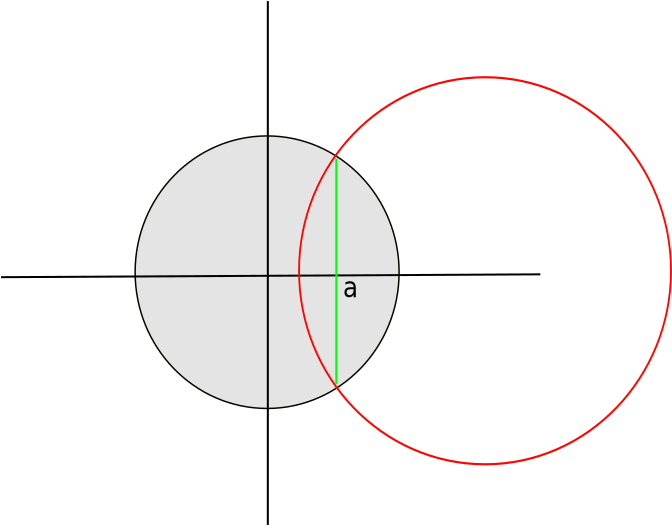
\includegraphics[width=6cm]{disk}
\caption{Poincare disk}
\end{minipage}
  \begin{minipage}[b]{8cm}\centering
 \includegraphics[width=6.5cm]{Poincare-upper}
 \caption{Hyperboloid and Poincare disk}
\end{minipage}
\end{figure}


\begin{figure}[h]
\centering
 \includegraphics[width=\textwidth]{triangle-upper}
 \caption{triangle in the upper half plane}
\end{figure}



\end{document}

